% Figure de l'echelle signee : cinq zones de largeur egale et cinq paires avec << I drink milk >>.
\definecolor{scalepos}{HTML}{0072B2}
\definecolor{scaleneg}{HTML}{D55E00}
\definecolor{scalemid}{HTML}{999999}
\begin{figure}[t]
\centering
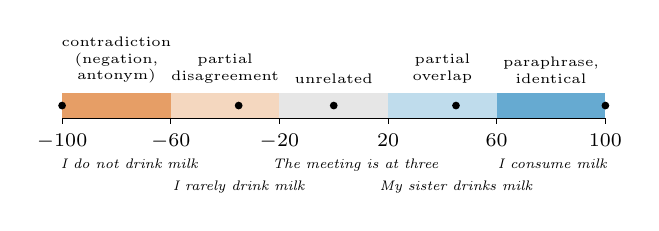
\begin{tikzpicture}[x=0.0345cm, y=1cm, font=\scriptsize]
  % palette symetrique : meme intensite de part et d'autre de zero
  \fill[scaleneg!60] (-100,0) rectangle (-60,0.32);
  \fill[scaleneg!25] (-60,0) rectangle (-20,0.32);
  \fill[scalemid!25] (-20,0) rectangle (20,0.32);
  \fill[scalepos!25] (20,0) rectangle (60,0.32);
  \fill[scalepos!60] (60,0) rectangle (100,0.32);
  \begin{scope}[every node/.style={above, align=center, font=\tiny}]
    \node at (-80,0.32) {contradiction\\(negation,\\antonym)};
    \node at (-40,0.32) {partial\\disagreement};
    \node at (0,0.32) {unrelated};
    \node at (40,0.32) {partial\\overlap};
    \node at (80,0.32) {paraphrase,\\identical};
  \end{scope}
  \draw (-100,0) -- (100,0);
  \foreach \v in {-100,-60,-20,20,60,100} {
    \draw (\v,0) -- (\v,-0.08);
    \node[below] at (\v,-0.08) {$\v$};
  }
  % paires construites sur << I drink milk >>, etiquettes sur deux rangees
  \foreach \v in {100, 45, 0, -35, -100} {
    \fill (\v,0.16) circle (1.4pt);
  }
  \begin{scope}[every node/.style={font=\tiny\itshape}]
    \node[below right, xshift=-4pt, yshift=-9pt] at (-100,-0.08) {I do not drink milk};
    \node[below, yshift=-17pt] at (-35,-0.08) {I rarely drink milk};
    \node[below, yshift=-9pt] at (8,-0.08) {The meeting is at three};
    \node[below, yshift=-17pt] at (45,-0.08) {My sister drinks milk};
    \node[below left, xshift=4pt, yshift=-9pt] at (100,-0.08) {I consume milk};
  \end{scope}
\end{tikzpicture}
\caption{The signed scale, with indicative zones. Dots: pairs formed with ``I drink milk''.}
\label{fig:scale}
\end{figure}
